\documentclass[a4paper, 11pt]{article}
\usepackage{comment} % enables the use of multi-line comments (\ifx \fi) 
\usepackage{lipsum} %This package just generates Lorem Ipsum filler text. 
\usepackage{fullpage} % changes the margin

\usepackage[T1]{fontenc}
\usepackage[english]{babel}
\usepackage[utf8]{inputenc}
\usepackage{lmodern}
\selectlanguage{english}
\usepackage{graphicx}
\usepackage{float}



\begin{document}
\noindent
\large\textbf{Post-Lab Multiscale Report} \hfill \textbf{Krzysztof Belcarz} \\
 \hfill Raport Date: 13/11/18 

\section*{Language}
Simulation of grain growth was implemented using C$\#$ language. Being high-level and deeply object oriented language it allows user to implement sophisticated and quite complicated algorithms relatively fast. What is more it supports numerous libraries used for data structures manipulation, as well as, computations of various kinds. Finally and probably this is the most important reason C Sharp allows user to create flexible and extensible graphical user interface utilizing "drag and drop" method, withoud the need to import any external libraries. As is commonly known 
fusing multiple technologies often causes complications, thus it is both time and resource consuming.
\section*{Graphical User Interface}
Program's graphical user interface is presented in figure \ref{GUI}
\begin{figure}[H]
\centering
  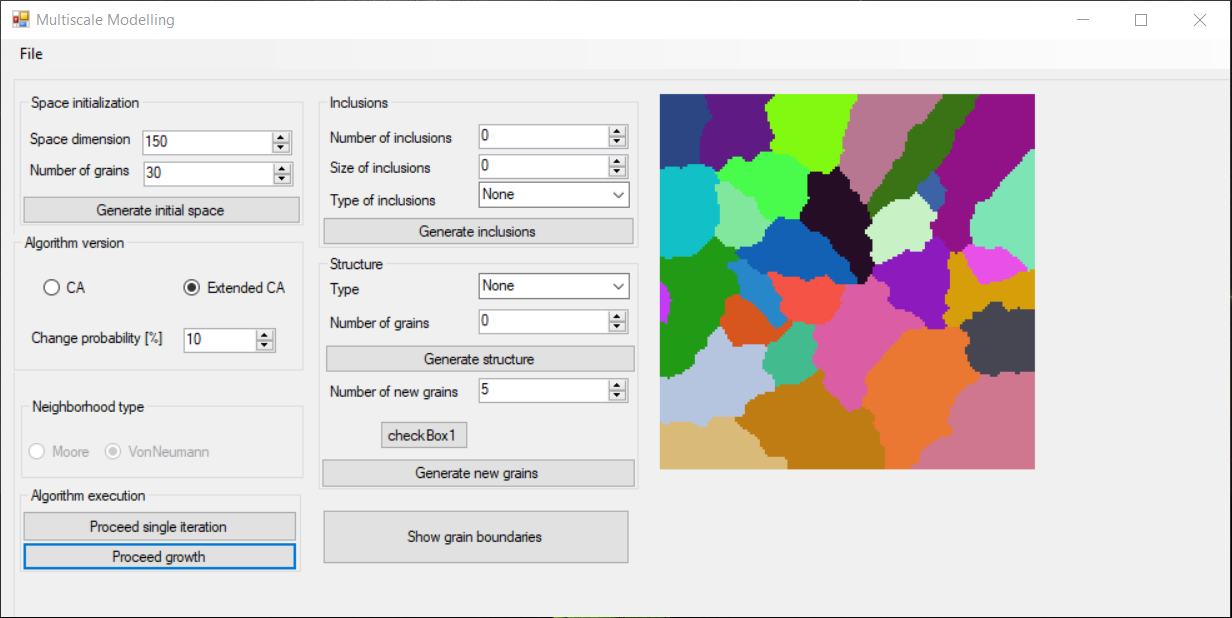
\includegraphics[width=\linewidth]{GUI}
  \caption{GUI}
  \label{GUI}
  \label{fig:boat1}
\end{figure}
In order to proceed with any algorithm one needs to generate space of desired size with inputted number of grains, as is depicted in \ref{SpaceInitLabel}
\begin{figure}[H]
\centering
  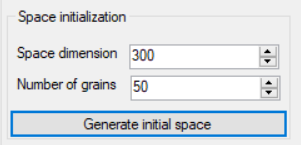
\includegraphics{SpaceInit}
  \caption{Space initialization group box}
  \label{SpaceInitLabel}
\end{figure}
\section*{Class 1 - Simple grain growth}
During first class the task was to implement basic version of Cellular Automata algorithm with utilizing classic Moore and VonNeumann neighborhood types. In order to ensure correct algorithm operation absorbing boundary condition was introduced. The state of cells on the edges of solution space were fixed with a specific value (0 in particular), thus they are not taken into account when updating grain structure.

In algorithm version group box \textbf{CA} radio button must be checked, as is shown in figure \ref{SimpleCALabel}
\begin{figure}[H]
\centering
  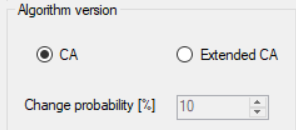
\includegraphics{SimpleCAGroupBox}
  \caption{Simple CA}
  \label{SimpleCALabel}
  \label{fig:boat1}
\end{figure}

After the growth utilizing simple CA is complete a space such as the one presented in \ref{SimpleCAExample} is produced.
\begin{figure}[H]
\centering
  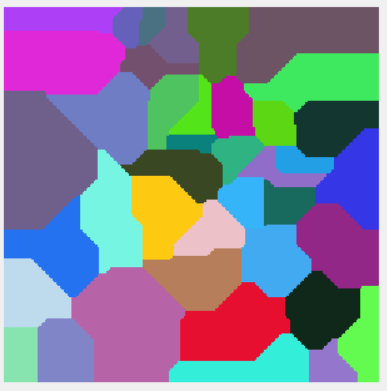
\includegraphics[]{SimpleCAExample}
  \caption{Example of simple CA algorithm}
  \label{SimpleCAExample}
\end{figure}


\section*{Class 2 - Microstructure import/export}
Second class goal was to implement mechanism of importing/exporting grain structure from/to file. In order to do so one shall access \textbf{File->Export data} or \textbf{File->Import data} depending on intentions, figure \ref{FileLabel}.
\begin{figure}[H]
\centering
  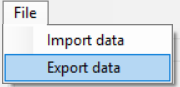
\includegraphics{File}
  \caption{Import/export menu}
  \label{FileLabel}
\end{figure}
\subsection{Exporting state}
State is saved simultaneusly in a bitmap and in a text file. User is able to choose the location where the files are supposed to be stored. Name for each file is generated automatically and is unique, because of the fact that it includes current date. Dialog corresponding to described functionality is presented in figure \ref{ExportToLabel}

\begin{figure}[H]
\centering
  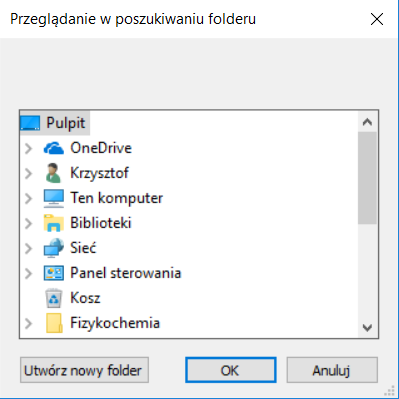
\includegraphics[]{ExportTo}
  \caption{Export dialog}
  \label{ExportToLabel}
\end{figure}

\subsubsection{Exporting state to bitmap}
\subsubsection{Exporting state to .txt file}

\subsection{Importing state}
In order to import state from a file one should choose proper file using dialog, such as the on in figure \ref{ImportLabel}.
\begin{figure}[H]
\centering
  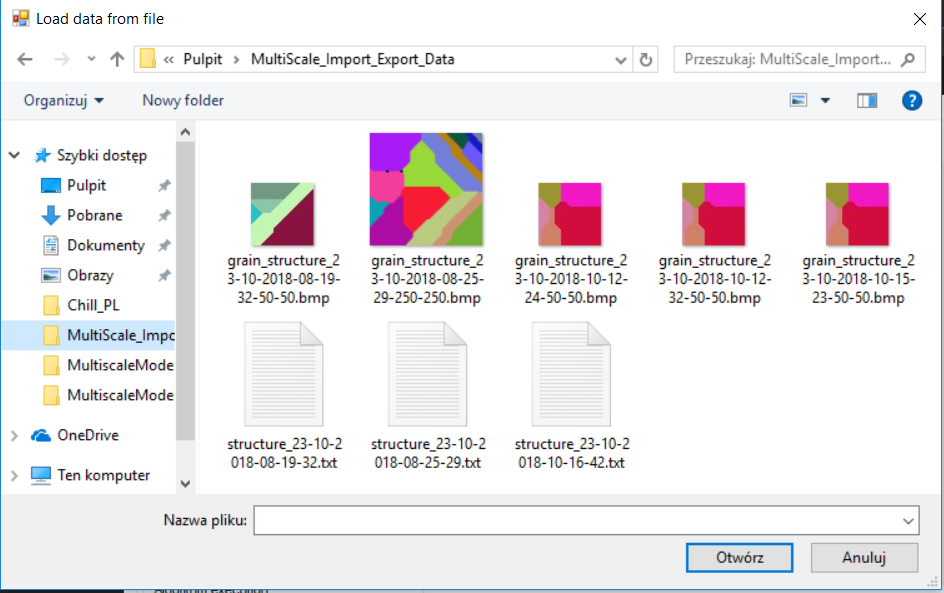
\includegraphics[width=\linewidth]{ImportFrom}
  \caption{Import dialog}
  \label{ImportLabel}
\end{figure}

\subsubsection{Importing state from .txt file}
The format of txt file is as follows:
\begin{enumerate}
\item Dimension of space
\item Header
\item Values corresponding to header's columns
\end{enumerate}
Example of such file can be observed in figure \ref{ExportedTxtLabel}:
\begin{figure}[H]
\centering
  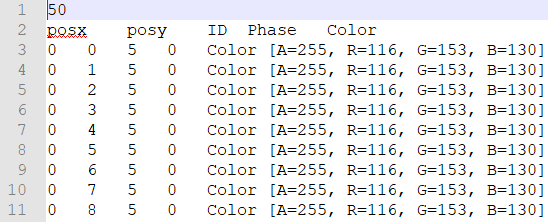
\includegraphics[]{ExportedTxt}
  \caption{structure$\_$23-10-2018-08-19-32.txt}
  \label{ExportedTxtLabel}
\end{figure}
\subsubsection{Importing state from bitmap}
Example of state imported from bitmap is presented in figure \ref{ExportedBitmapLabel}
\begin{figure}[H]
\centering
  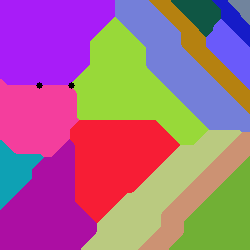
\includegraphics[]{ExportedBitmap}
  \caption{grain$\_$structure$\_$23-10-2018-08-25-29-250-250.bmp}
  \label{ExportedBitmapLabel}
\end{figure}

\section*{Class 3 - Inclusions}
Aim of next class was to introduce a feature which would allow user to add inclusions to grain structure either before the growth (in any place/coordinates) or after the growth (only on grain borders).
Inclusions are defined with following parameters:
\begin{itemize}
\item number - how many inclusions to create
\item size - what is the diameter (circular)/ side (square) of a single inclusion
\item type - what type of inclusions to create (circular/square)
\end{itemize}
A callback function is connected to structure display space, so that user can click and add inclusions of his/her choosing before the growth starts and a dedicated button is responsible for generating inclusions specified with parameters in corresponding group box is also available.\newline
Any action will take place only when type of inclusion is changed to a valid one (from default None) and automatic generation will take place only when number of inclusions is positive, as well as, their size. Mentioned inclusion group box example is in figure \ref{InclusionsGroupBoxLabel}.
\begin{figure}[H]
\centering
  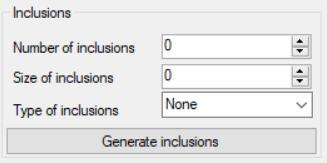
\includegraphics[]{InclusionsGroupBox}
  \caption{Inclusions group box}
  \label{InclusionsGroupBoxLabel}
\end{figure}


Example of structure with circular inclusions can be seen in \ref{CircularInclusionsExampleLabel}
\begin{figure}[H]
\centering
  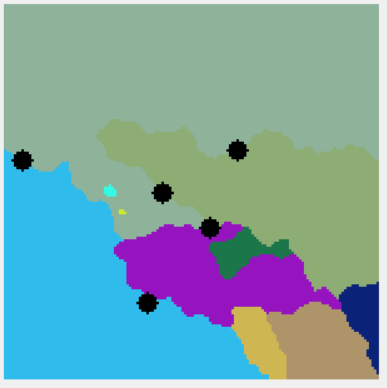
\includegraphics[]{CircularInclusionsExample}
  \caption{Example of circular inclusions}
  \label{CircularInclusionsExampleLabel}
\end{figure}

Example of structure with square inclusions can be seen if \ref{SquareInclusionsExampleLabel}:
\begin{figure}[H]
\centering
  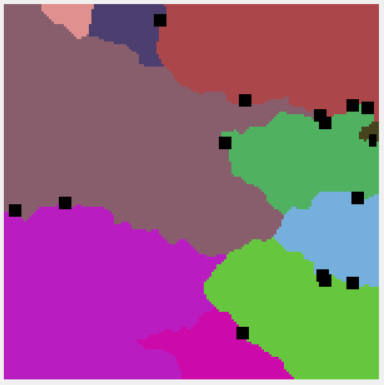
\includegraphics[]{SquareInclusionsExample}
  \caption{Example of square inclusions}
  \label{SquareInclusionsExampleLabel}
\end{figure}
\section*{Class 4 - Extended CA}
Fourth class purpose was to implement extended version of Cellular Automata algorithm. Instead of one rule used in basic four rules were implemented, featuring new types of neighborhoods, as well as, new conditions for changing state of a particular cell.

In order to take adventage of extended version of the algorithm it must be checked on algorithm version group box, as presented in \ref{ExtendedCAGroupBoxLabel}:
\begin{figure}[H]
\centering
  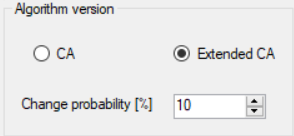
\includegraphics{ExtendedCAGroupBox}
  \caption{Extended CA}
  \label{ExtendedCAGroupBoxLabel}
\end{figure}
Then and only then probability parameter for 4th rule is unlocked for modification.

After the growth utilizing extended CA is complete a space such as the one presented in \ref{ExtendedCAExampleLabel} is produced.
\begin{figure}[H]
\centering
  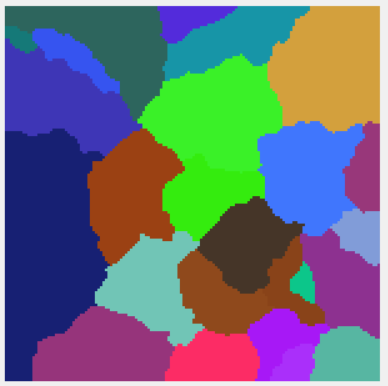
\includegraphics[]{ExtendedCAExample}
  \caption{Example of extended CA algorithm}
  \label{ExtendedCAExampleLabel}
\end{figure}



\section*{Class 5 - Substructures/Dual phase}
In course of class number 5 we were supposed to give user possibility to create a substructure or dual phase after initial growth. User can choose how many grains from initial growth are meant to be considered while creating substructure of dual phase. After those grains are ''transformed'' according to user preference new grains can be added and once more growth is possible.
\subsection{Substructure}
User defined number of grains is preserved on the space with their original color and IDs. Example can be observed in figure \ref{SubstructureExampleLabel}.
\begin{figure}[H]
\centering
  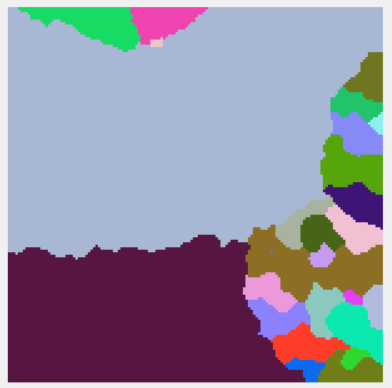
\includegraphics[]{SubstructureExample}
  \caption{Example of a substructure}
  \label{SubstructureExampleLabel}
\end{figure}
\subsection{Dual phase}
User defined number of grains is preserved on the space with a new color common for all of them and their phase parameter is incremented. Exemplary space is shown in figure \ref{DualPhaseExampleLabel}.
\begin{figure}[H]
\centering
  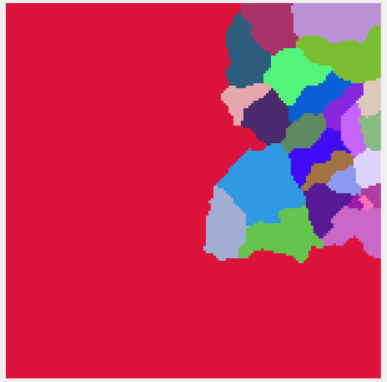
\includegraphics{DualPhaseExample}
  \caption{Example of dual phase}
  \label{DualPhaseExampleLabel}
\end{figure}
\section*{Class 6 - Grain boundaries}
After the growth with chosen algorithm version is complete user can generate grain boundaries and display them, as is presented in \ref{GrainBoundariesExampleLabel}
\begin{figure}[H]
\centering
  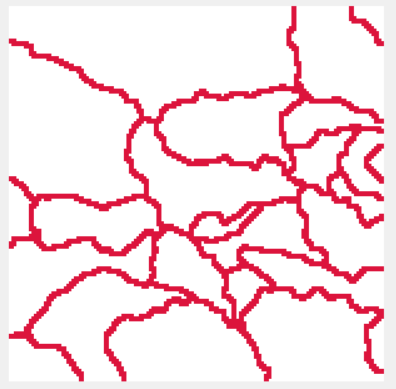
\includegraphics[]{GrainBoundariesExample}
  \caption{Example grain boundaries}
  \label{GrainBoundariesExampleLabel}
\end{figure}

\section*{Comparison of generated results with real microstructures}
As it can be clearly seen in figures \ref{Comparison1Label}, \ref{Comparison2Label}, \ref{Comparison3Label} real microstructures (left side of comparison pictures) and the ones generated using implemented simulation program (right side of comparison pictures) differ in the context of grain sizes and their shapes, however they are coherent in the context of general look.  
\begin{figure}[H]
\centering
  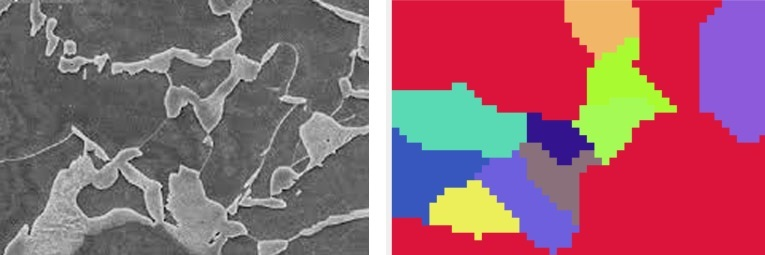
\includegraphics[width=\textwidth]{Comparison1}
  \caption{Comparison picture 1}
  \label{Comparison1Label}
\end{figure}

\begin{figure}[H]
\centering
  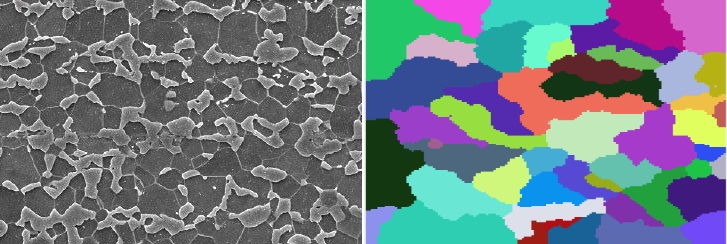
\includegraphics[width=\textwidth]{Comparison2}
  \caption{Comparison picture 2}
  \label{Comparison2Label}
\end{figure}

\begin{figure}[H]
\centering
  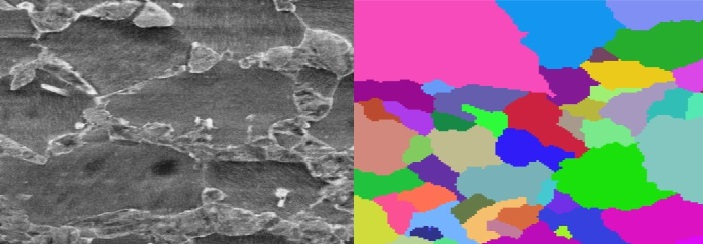
\includegraphics[width=\textwidth]{Comparison3}
  \caption{Comparison picture 3}
  \label{Comparison3Label}
\end{figure}


\section*{Conclusions}
Right now due to numerous features being based on pseudo random distributions or locations the algorithm work can be controlled only to a certain degree. Because of that fact it is possible to obtain higher level of similarity to real structures, but it could be very time consuming. In order to make the program even more useful one could implement a number of features, such as:
\begin{itemize}
\item[•] possibility to choose arbitrarily placement of grains
\item[•] possibility to change shape of a particular grain after growth(e.g. by drag and drop of it's boundary)
\item[•] possibility to copy/paste a fragment of structure in a "fractal-like" manner
\end{itemize}

In general all part of the project were successfully implemented and none of them caused problem, however quite a few were challenging. For a software engineer who works mostly with algorithm implementation and not with GUIs it's a refreshing experience to deal with all issues emerging from user interactions. It definitely allowed to widen the knowledge regarding both the mechanism of grain growth and C Sharp programming.
\section*{Attachments}
All source files as well as pdf version of the raport are accessible through repository:
https://github.com/krsonetbg/MultiscaleModelling
%Make sure to change these
%Lab Notes, HelloWorld.ic, FooBar.ic
%\fi %comment me out


\end{document}
